\documentclass[11pt]{article}

\usepackage{geometry}
\geometry{
  a4paper,
  total={170mm,257mm},
  left=20mm,
  top=20mm,
}

\usepackage{amsmath}
\usepackage{hyperref}
\usepackage{graphicx}

\newcommand{\figplaceholder}[2]{%
  \begin{figure}[ht]
  \centering
  \fbox{\rule{0pt}{2.4in}\rule{0.9\linewidth}{0pt}}
  \caption{#2}
  \label{#1}
  \end{figure}
}

\title{Lagrangian Plume Trajectory Tools: Backward Source Attribution and Forward Dispersion}
\author{Alexander Ukhov, Ibrahim Hoteit}
\date{KAUST, December 2025}

\begin{document}
\maketitle

\section{Motivation and Scope}
Volcanic eruption monitoring relies on both source attribution (when and how high
the material was injected) and forward dispersion (where the material travels
after release). This repository provides two complementary Lagrangian tools
built on WRF winds:
\begin{itemize}
  \item \textbf{Backward source attribution} with \texttt{plume\_backtraj.py}:
        start from a satellite-retrieved column and trace parcels backward to a
        receptor cylinder around the vent, producing a time--height emission
        scenario.
  \item \textbf{Forward dispersion} with \texttt{plume\_forwtraj.py}: release a
        vertical column of parcels at the source and advect them forward to map
        transport pathways and ages.
\end{itemize}
Optional physics includes aerosol settling and (for SO$_2$) backward mass
correction with an e-folding lifetime.

\section{Inputs and Configuration}
\subsection{WRF meteorology}
Both workflows require one or more WRF \texttt{wrfout} files containing grid
geometry (\path{XLAT}, \path{XLONG}, \path{DX}, \path{DY}, map factors), winds
(\path{U}, \path{V}, \path{W}), geopotential (\path{PH}, \path{PHB}), and
\path{Times}. When multiple files are supplied they are assumed to be ordered in
time (or provided via a sortable wildcard).

\subsection{Column field for backward runs}
Backward runs ingest a 2-D column field on the WRF grid (e.g.\ SO$_2$ column or
UV aerosol index) provided via \path{--column}. The field is read from a NetCDF
variable specified by \path{--column-var} and optionally scaled by
\path{--column-coef}. A plume mask is created using \path{--threshold}; parcels
are seeded only where the column exceeds the threshold (and optionally within
\path{--seed-bbox}). The time index is selected from \path{--start-time} (nearest
WRF time), and plot labels can be customized with \path{--colorbar-label}.

\subsection{Source specification for forward runs}
Forward runs require a source location or a bounding box:
\begin{itemize}
  \item \path{--source-lat}, \path{--source-lon} for a single column, or
  \item \path{--seed-bbox} with \path{--n-columns} for random source columns.
\end{itemize}
Parcels are initialized between \path{--z-min} and \path{--z-max} with
\path{--n-vert} samples. The run spans \path{--start-time} to \path{--end-time},
with a sub-step \path{--integration-dt} in seconds.

\section{Backward Lagrangian Source Attribution (\texttt{plume\_backtraj.py})}
\subsection{Parcel initialization}
The column field is thresholded to define a plume mask. A user-specified number
of grid cells (\path{--n-columns}) are sampled from the mask, and at each sampled
cell a vertical line of parcels (\path{--n-vert}) is created with random heights
between \path{--z-min} and \path{--z-max}. Each parcel carries a weight derived
from the column field, enabling both count-based and mass-weighted diagnostics.

\subsection{Backward advection}
Parcel positions are integrated backward in time using a fourth-order
Runge--Kutta scheme with winds interpolated in space and time (sub-step
\path{--integration-dt}). Parcels are deactivated when they leave the domain,
reach the eruption start time (\path{--emission-start}), or enter the receptor
cylinder.

\subsection{Receptor diagnostics and emission matrix}
The receptor is a vertical cylinder around the vent, defined by
\path{--receptor-lat}, \path{--receptor-lon}, \path{--receptor-radius}, and
\path{--receptor-min-h}--\path{--receptor-max-h}. Parcel arrivals are binned on
a time--height grid with \path{--arrival-bin-minutes}. If both
\path{--emission-start} and \path{--emission-end} are supplied, fixed time bins
spanning the eruption window are used and arrivals outside the window are
ignored.

\subsection{Mass weighting and SO$_2$ decay}
Mass-weighted outputs use the column value multiplied by cell area and divided
by \path{--n-vert}. If \path{--so2-efolding-days} is set, parcel masses are
adjusted backward in time using an exponential correction to compensate for SO$_2$
oxidation.

\subsection{Reproducibility}
All inputs and outputs can be serialized to a pickle file using
\path{--state-pickle}. The file includes grid data, trajectories, emission
matrices, and metadata so plots can be reproduced without re-running the solver.

\section{Forward Lagrangian Dispersion (\texttt{plume\_forwtraj.py})}
\subsection{Parcel release}
Parcels are released either from a single source column or multiple columns
randomly sampled inside \path{--seed-bbox}. Each column contains
\path{--n-vert} parcels between \path{--z-min} and \path{--z-max}.


\subsection{Ash gravitational settling}

The gravitational settling of aerosols is a key driver of their removal from the atmosphere. The modeled volcanic ash is subdivided into different bins representing the size spectrum of the particles. In WRF-Chem, ash particles are categorized into 10 size bins based on their radii, ranging from 0.01955 to 1000.0 µm, see Table \ref{tab:particle_size_divided}. For the ash gravitational settling, the terminal velocities are calculated for the mean arithmetic radii ($R_{m}$) within each bin size. Ash density is assumed to be 2500 \unit{kg\ m^{-3}}, see Table \ref{tab:particle_size_divided}.


\begin{table}[b!]
\centering
\begin{tabular}{|c|c|c|c|c|}
\hline
Bin & Radius lower bound (µm) & Radius upper bound (µm) & $R_\text{m}$ (µm) & Density (\unit{kg\ m^{-3}}) \\ \hline
ash1 & 500 & 1000 & 500 & 2500 \\
ash2 & 250 & 500 & 375 & 2500 \\
ash3 & 125 & 250 & 187.5 & 2500 \\
ash4 & 62.5 & 125 & 93.75 & 2500 \\
ash5 & 31.25 & 62.5 & 46.88 & 2500 \\
ash6 & 15.625 & 31.25 & 23.44 & 2500 \\
ash7 & 7.8125 & 15.625 & 11.72 & 2500 \\
ash8 & 3.90625 & 7.8125 & 5.86 & 2500 \\
ash9 & 1.95325 & 3.9065 & 2.93 & 2500 \\
ash10 & 0.01955 & 1.95325 & 0.97 & 2500 \\ \hline
\end{tabular}
\caption{Ash particle bin size ranges with corresponding WRF-Chem ash bins.}
\label{tab:particle_size_divided}
\end{table}



\subsection{Forward advection and optional settling}
Parcels are advected forward in time using the same RK4 integration approach as
the backward solver, with spatial and temporal interpolation of WRF winds. For
aerosol types (e.g.\ \path{sulf}, \path{ash1}--\path{ash10}) a settling velocity
profile can be added using \path{--aer-type}.

\begin{figure}[t!]
    \centering
    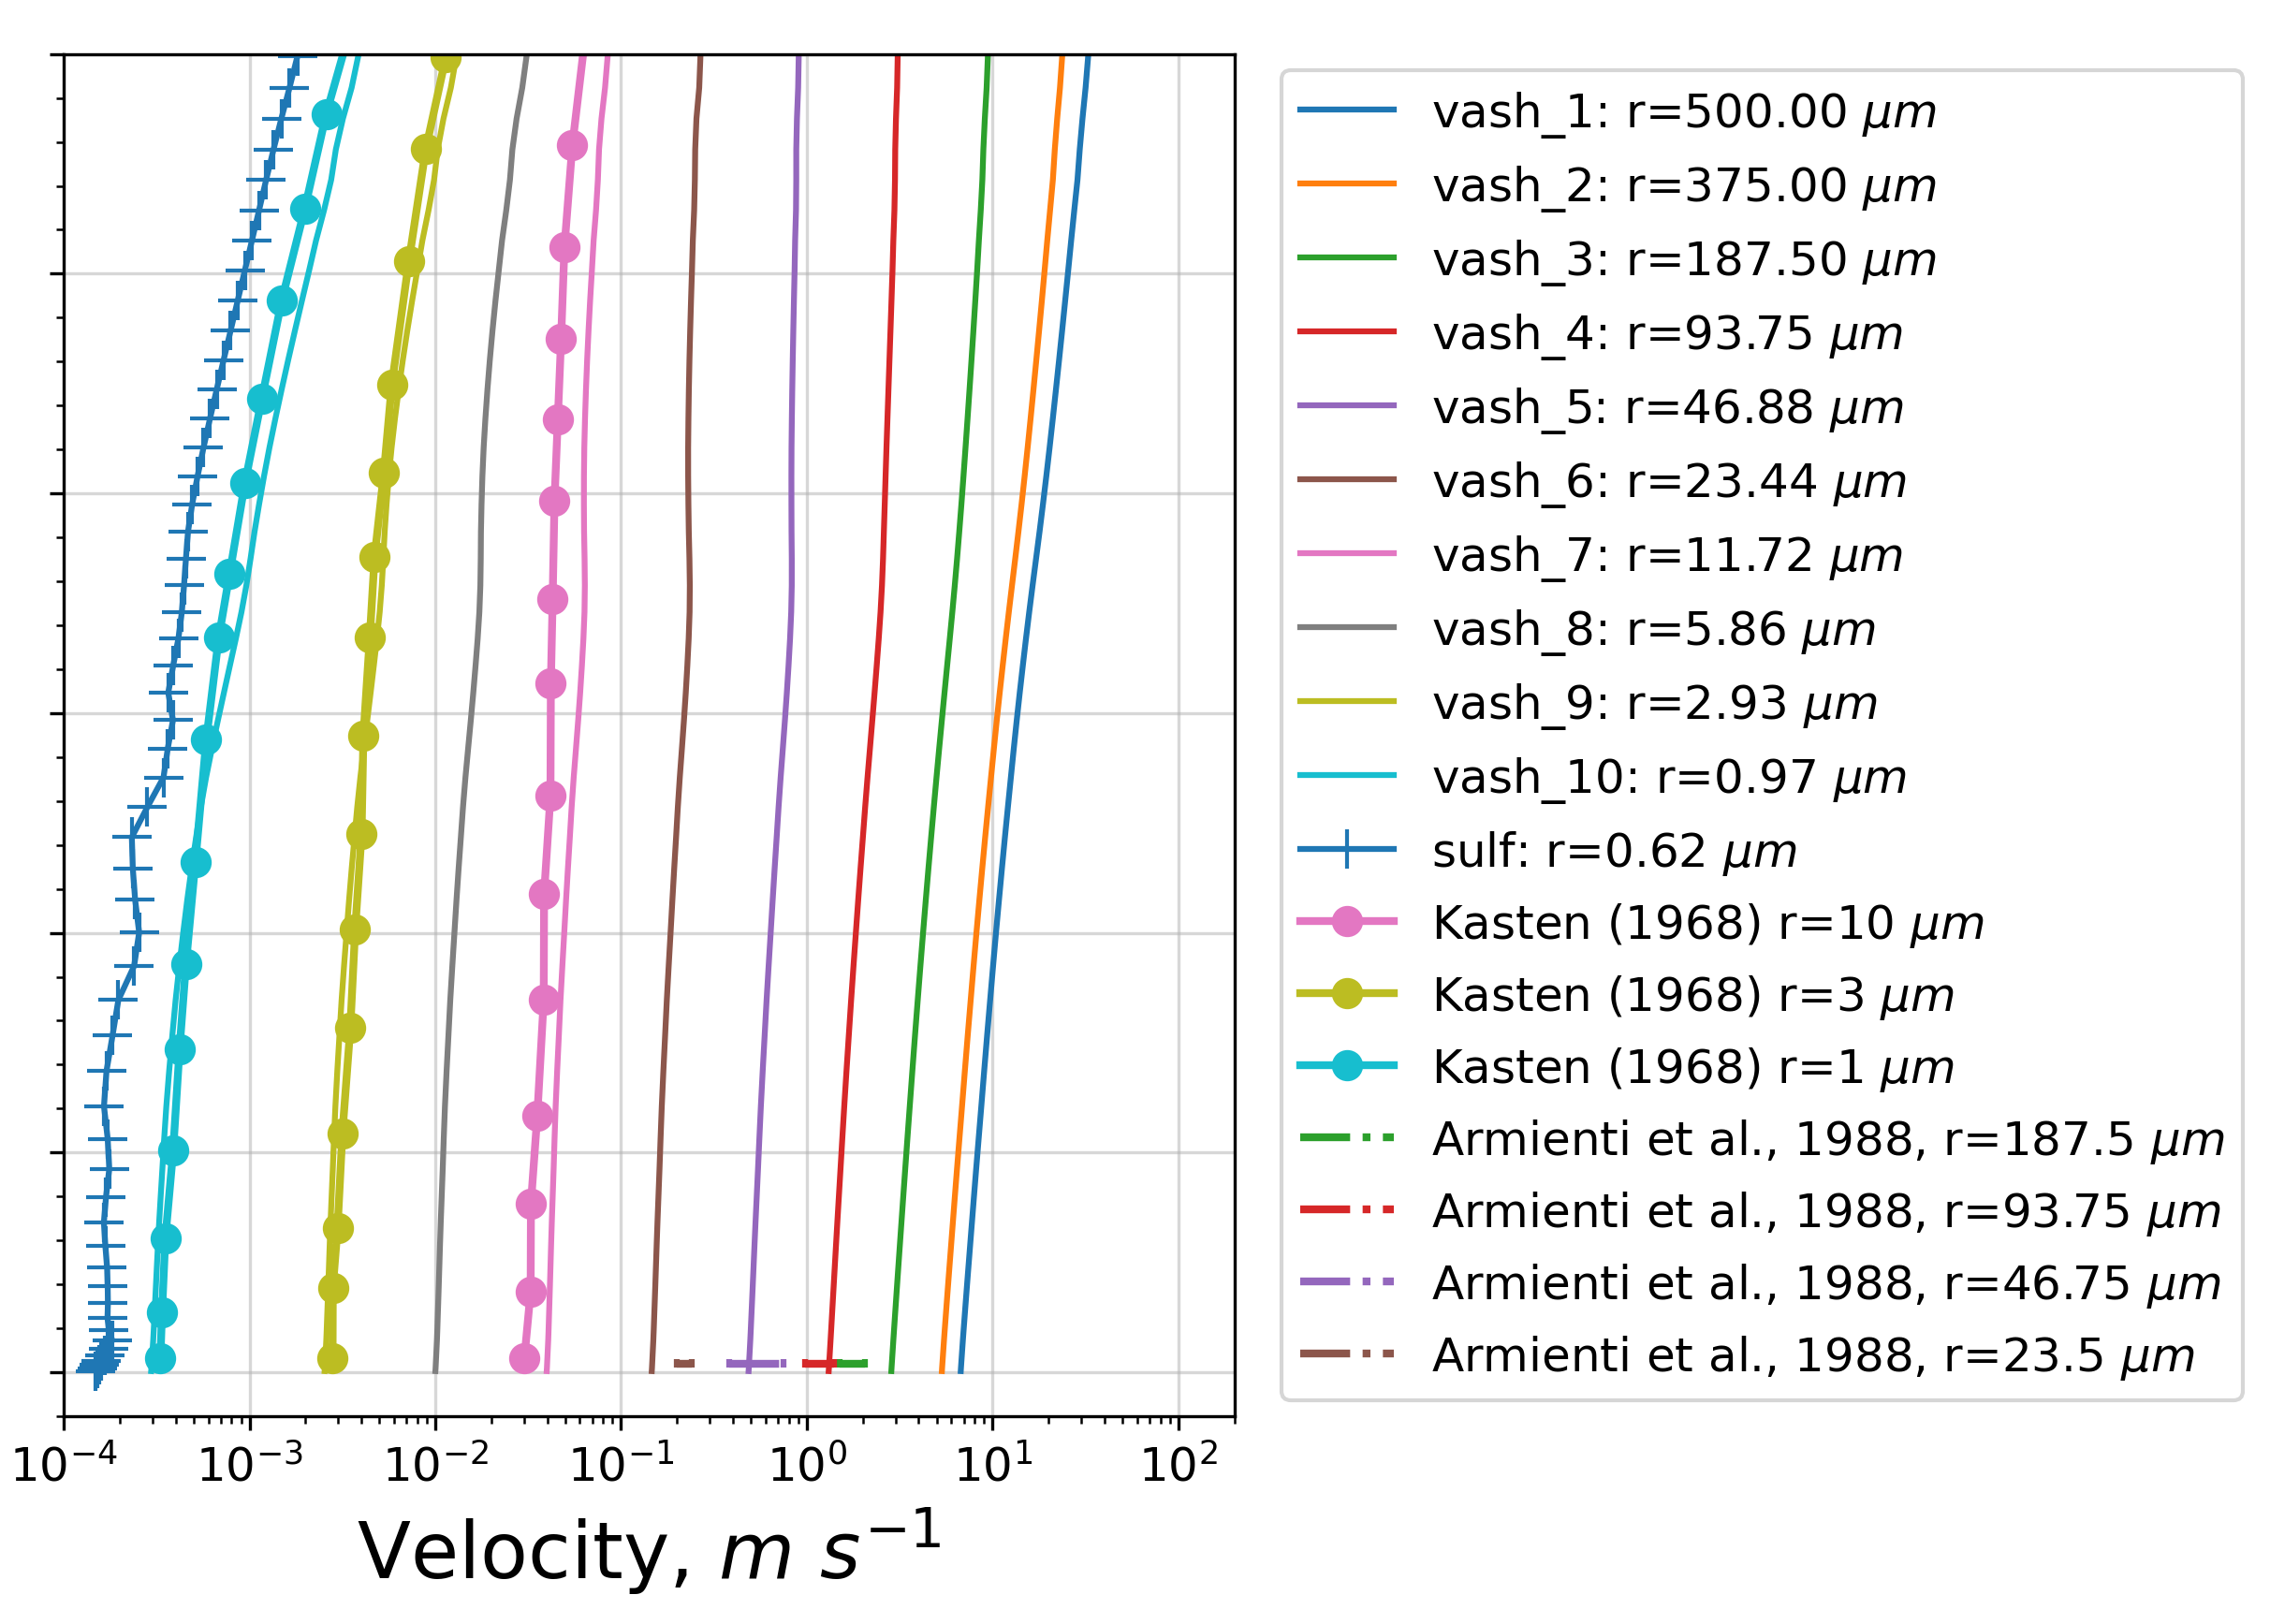
\includegraphics[width=1.0\linewidth]{./Fig1.png}
    \caption{Settling velocity as a function of altitude computed for ash
    particles with different radii and sulfate particles with dry volume median
    radii = 0.62~$\mu$m. Comparison with theoretical data by
    \cite{kasten1968falling} and \cite{armienti1988numerical}.}
    \label{fig:grav_settl_velocities}
\end{figure}

Figure \ref{fig:grav_settl_velocities} illustrates the settling velocities of
ash particles as a function of altitude for multiple particle radii. The
gravitational settling velocity of sulfate particles having dry volume median
radii = 0.62~$\mu$m is also shown. We compare our results with theoretical
formulations by \cite{kasten1968falling} and \cite{armienti1988numerical}. In
\cite{kasten1968falling}, settling velocities are for spherical particles with
radii of 1~$\mu$m, 3~$\mu$m, and 10~$\mu$m; for comparison, the density of these
particles was adjusted to align with that of ash. In
\cite{armienti1988numerical}, ranges of terminal velocities are provided for
feldspar mineral particles (radii of 23.5~$\mu$m, 46.75~$\mu$m, 93.75~$\mu$m,
and 187.5~$\mu$m), which are regarded as having the closest density to ash
particles.

Settling velocities increase with particle size and with altitude. Sulfate
particles, possessing lower density and smaller size, exhibit the minimal
settling velocity. The corresponding curve appears irregular compared with the
smoother curves for ash particles due to water uptake affecting the size and,
therefore, settling velocity of sulfate particles.

\subsection{Stopping conditions and state export}
Parcels stop when they exit the WRF domain. A \path{--state-pickle} can be
written to allow later re-plotting of height- and age-colored trajectories.

\section{Output Files and Formats}
\subsection{Backward emission matrices}
Two TXT files can be produced: a count-based matrix (\path{--output-txt}) and an
optional mass-weighted matrix (\path{--mass-output-txt}). The format is:
\begin{verbatim}
time <label_1> <label_2> ...
height <z_1> <z_2> ...
<row for top height bin>
...
\end{verbatim}
Time labels are absolute datetimes when WRF times are available and an emission
reference is supplied; otherwise they are numeric offsets.

\subsection{Forward trajectory outputs}
Forward runs write height-colored and age-colored trajectory maps
(\path{--height-figure}, \path{--age-figure}) and may include a vertical seed
distribution plot (\path{--seeds-vertical-figure}).

\section{Figure Placeholders}
The following placeholders cover all image products produced by the workflow
and helper scripts. All plotting commands accept \path{--map-extent} to override
map bounds when needed.

\subsection{Backward-run figures}
\figplaceholder{fig:back-seeds}{Initial parcel locations on the column field
(\path{--seeds-figure}).}
\figplaceholder{fig:back-seeds-vertical}{Initial vertical parcel distribution
(\path{--seeds-vertical-figure}).}
\figplaceholder{fig:back-hourly}{Hourly parcel snapshots during backward advection
(\path{--hourly-figures}, representative frame).}
\figplaceholder{fig:back-trajectories}{Trajectories reaching the receptor, colored
by initial height (\path{--trajectory-figure}).}
\figplaceholder{fig:back-trajectory-age}{Trajectories colored by parcel age at
receptor (\path{--trajectory-age}).}
\figplaceholder{fig:back-trajectory-emission-time}{Trajectories colored by emission
time since \path{--emission-start} (\path{--trajectory-emission-time-figure}).}
\figplaceholder{fig:back-trajectory-arrival-height}{Trajectories colored by
arrival height in the receptor cylinder
(\path{--trajectory-arrival-height-figure}).}
\figplaceholder{fig:back-missed}{Trajectories that never reached the receptor
(\path{--missed-trajectory-figure}).}
\figplaceholder{fig:back-emission-matrix}{Emission time--height matrix of parcel
counts (\path{--output-figure}).}
\figplaceholder{fig:back-mass-matrix}{Mass-weighted emission matrix
(\path{--mass-figure}).}

\subsection{Forward-run figures}
\figplaceholder{fig:forw-height}{Forward trajectories colored by parcel height
(\path{--height-figure}).}
\figplaceholder{fig:forw-age}{Forward trajectories colored by parcel age
(\path{--age-figure}).}
\figplaceholder{fig:forw-seeds-vertical}{Initial vertical parcel distribution for
forward runs (\path{--seeds-vertical-figure}).}

\subsection{Aggregation figures (optional)}
The aggregation utilities in \path{misc/} replot combined diagnostics from
multiple pickles.
\figplaceholder{fig:agg-back-trajectories}{Aggregated backward trajectories
(\path{aggregated\_trajectories.png}).}
\figplaceholder{fig:agg-back-seeds}{Aggregated parcel locations
(\path{aggregated\_parcel\_locations.png}).}
\figplaceholder{fig:agg-back-trajectory-age}{Aggregated trajectory age map
(\path{aggregated\_trajectory\_ages.png}).}
\figplaceholder{fig:agg-back-trajectory-emission-time}{Aggregated emission-time
map (\path{aggregated\_trajectory\_emission\_time.png}).}
\figplaceholder{fig:agg-back-trajectory-arrival-height}{Aggregated arrival-height
map (\path{aggregated\_trajectory\_arrival\_height.png}).}
\figplaceholder{fig:agg-back-missed}{Aggregated missed trajectories
(\path{aggregated\_missed\_trajectories.png}).}
\figplaceholder{fig:agg-back-emission}{Aggregated emission matrix
(\path{aggregated\_emission\_matrix.png}).}
\figplaceholder{fig:agg-back-mass}{Aggregated mass-weighted emission matrix
(\path{aggregated\_mass\_matrix.png}).}
\figplaceholder{fig:agg-forw-height}{Aggregated forward trajectories colored by
height (\path{plume\_height\_colored\_aggregate.png}).}
\figplaceholder{fig:agg-forw-age}{Aggregated forward trajectories colored by age
(\path{plume\_age\_colored\_aggregate.png}).}
\figplaceholder{fig:agg-forw-seeds-vertical}{Aggregated forward vertical seed
distribution (\path{seeds\_vertical\_aggregate.png}).}

\section{Re-plotting and Aggregation}
\texttt{plot\_backtraj.py} and \texttt{plot\_forwtraj.py} regenerate the same
figure types from a saved \path{--state-pickle}. The aggregation scripts
\texttt{misc/aggregate\_backtraj.py} and \texttt{misc/aggregate\_forwtraj.py}
combine multiple pickles and output the aggregated figures listed above.

\section{Coupling to PrepEmisSources}
The backward emission matrices provide a direct bridge to the emission scenarios
used by \href{https://github.com/saneku/PrepEmisSources}{PrepEmisSources}. A
typical coupling workflow is:
\begin{enumerate}
  \item Run \texttt{plume\_backtraj.py} with \path{--emission-start} and
        \path{--emission-end} aligned to the WRF-Chem simulation window.
  \item Use the mass-weighted matrix (\path{--mass-output-txt}) as the
        time--height distribution of emitted mass; optionally normalize or scale
        it to match the desired total SO$_2$ or ash budget.
  \item Translate the matrix into the emission scenario format expected by
        PrepEmisSources, preserving the time bin edges and vertical structure.
\end{enumerate}
This links observed plume retrievals to physically consistent emission scenarios
that can be injected into WRF-Chem via PrepEmisSources
(\cite{Ukhov2025PrepEmis}).

\section{References}
\begin{thebibliography}{9}
\bibitem{Ukhov2025PrepEmis}
Ukhov, A., Stenchikov, G., Schnell, J., Ahmadov, R., Rizza, U., Grell, G., and
Hoteit, I.: Enhancing volcanic eruption simulations with the WRF-Chem v4.8,
Geosci.\ Model Dev., 18, 9805--9825,
\href{https://doi.org/10.5194/gmd-18-9805-2025}{https://doi.org/10.5194/gmd-18-9805-2025},
2025.

\bibitem{armienti1988numerical}
Armienti, P., Macedonio, G., and Pareschi, M.\ T.: A numerical model for
simulation of tephra transport and deposition: Applications to May 18, 1980,
Mount St.\ Helens eruption, J.\ Geophys.\ Res.: Solid Earth, 93(B6), 6463--6476,
1988.

\bibitem{kasten1968falling}
Kasten, F.: Falling speed of aerosol particles, J.\ Appl.\ Meteorol., 7(5),
944--947, 1968.
\end{thebibliography}

\end{document}
